\section{Results and Analysis}\label{6_results}
\begin{comment}
Each calculated variable was averaged across the three consecutive recorded trials.
Further, the data is provided as means with standard deviations.
A two-tailed paired-samples t-test was used to compare the single leg stance (seconds) and walking over the line performance (steps and cm) for the left and right leg before and after training.
For all pre to post variables the difference was calculated to test its normal distribution with the Shapiro-Wilk test and find outliers via boxplots in the dataset.
Because of the small number of subject all tests were verified with the non-parametric Wilcoxon signed ranks test.
An independent-samples t-test was conducted to compare the slackline performance in single leg stance (seconds) and walking over the line (steps and cm) for the left and right leg between the interactive system group and human trainer group.
For all post variables the normal distribution was calculated.
Further, the homogeneity of variance is calculated to meet the requirements of an independent t-test.
Like in the paired-sample t-test a non-parametric Mann-Whitney U test was used to verify the outcome of the independent t-test.
Level of significance was set at $p$ < 0.05.

As non-parametric testing revealed nearly identical results for all conditions as compared to the mixed ANOVA testing procedure, only the parametrical test results will be presented in a uniform manner.
Separate 2 x 2 mixed analysis of variance (mixed ANOVA) with one withing-group (time: Pre vs. Post) and one between-group (group: ISG vs. HTG) factor were calculated to test interaction effects of training, global differences in the dependent variables between pre and post, and possible differences between ISG and HTG.

Two-tailed independent t-test were used to determine possible PRE test differences between the ISG and HTG groups as well as POST test differences.
Further dependent t-tests for paired samples were used to test for differences in dependent variables between PRE and POST.
All outcomes were calculated for each variable separately.
Level of significance was set at p < 0.05.
Effect size was shown by using Cohen's $f$ (partial eta squared) and was defined as small for $f$>0.1, medium for $f$>0.25 and large for $f$>0.4 .
 calculated by the statistics software G*Power 3
\end{comment}

Data are provided as means with standard deviations.
Each calculated variable (for the left and right leg separately in single leg standing time, walked steps over the line, walked distance on the line) was averaged across the three consecutive recorded trials.
Separate 2 (group: ISG and HTG) x 2 (time: PRE and POST) mixed-design analysis of variance (mixed ANOVA) was performed.
To match the requirements of the mixed ANOVA, all parameters were tested on normality with the Shapiro-Wilk test.
Despite walking steps performance in the post measurement for the left and right foot, all data were normally distributed with $p$ > 0.05.
Further, the homogeneity of error variances was assessed by Levene's test with $p$ > 0.05 and the homogeneity of covariances were calculated by Box's test with $p$ > 0.05.
Given these requirements the mixed ANOVA was used for testing interaction effects with sphericity assumed since the group level is < 3, global differences in the dependent variables between PRE and POST, and possible differences between ISG and HTG.
Level of significance was set at $p$ < 0.05.
Effect size was shown by using partial eta squared ($\eta_{p}^{2}$) and was defined as small for $\eta_{p}^{2}$ $\geq$ 0.01, medium for $\eta_{p}^{2}$ $\geq$ 0.06, and large for $\eta_{p}^{2}$ $\geq$ 0.14.

As testing with removed and/or corrected outliers have not shown any essential difference in effects of significance, only the parametrical test results without any removed or corrected data will be shown, to present the results in a uniform manner.
All analyses were performed using SPSS Statistics version 25.

The measurement results can be seen in Table \ref{tab:6_4_results} and the results of the analysis in Table \ref{tab:6_4_mainEffects}.
In the following, the requirements and results of the mixed ANOVA testing will be reported for each condition separately as well as for the left and right leg.

\subsection{Single Leg Stance Performance}
The homogeneity of error variances was given for the single leg performance for the left and right leg, as assessed by Levene's test with $p$ > 0.05.
There was also homogeneity of covariances, as assessed by Box's test for the left ($p$ = 0.699) and right leg ($p$ = 0.601).

No statistically significant interaction effect between time and group has been found, for the left $F$(1.0, 10.0) = 0.069, p = 0.798, partial $\eta_{p}^{2}$ = 0.007 as well as for the right leg $F$(1.0, 10.0) = 0.004, p = 0.950, partial $\eta_{p}^{2}$ = 0.000 (see Figure \ref{fig:6_4_standImprovement}).
Since there was no significant interaction effect, the main effects will be reported.

There was no statistically significant main effect within-subjects for time (PRE to POST) for the left leg, $F$(1.0, 10.0) = 3.843, p = 0.078, partial $\eta_{p}^{2}$ = 0.278.
However, a large statistically significant main effect within-subjects for time (PRE to POST) was found for the right leg, $F$(1.0, 10.0) = 15.548, p = 0.003, partial $\eta_{p}^{2}$ = 0.609.

No significant main effect between-subjects for group (ISG to HTG) has been found for the left $F$(1.0, 10.0) = 0.009, p = 0.928, partial $\eta_{p}^{2}$ = 0.001 and right leg, $F$(1.0, 10.0) = 0.008, p = 0.931, partial $\eta_{p}^{2}$ = 0.001.
\begin{figure}[htb]
	\centering
	\begin{minipage}[t]{0.49\linewidth}
		\centering
		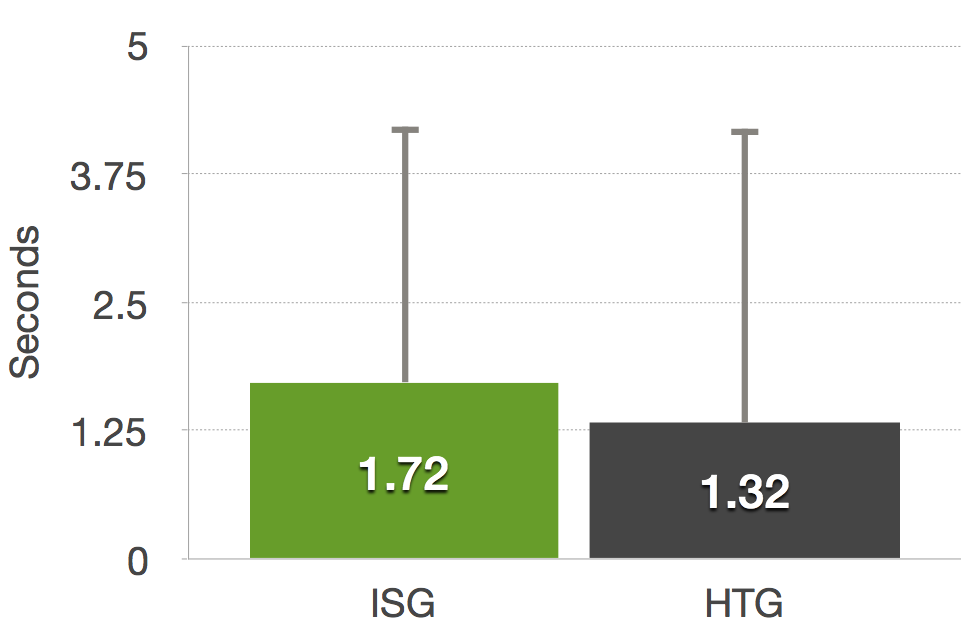
\includegraphics[width=1\linewidth]{Pictures/6_4_DIA_StandLeftDiff}
		\subcaption{Improvement on Standing with Left Leg}
		\label{fig:6_4_standLeftImprovement}
	\end{minipage}
	\hfill
	\begin{minipage}[t]{0.49\linewidth}
		\centering
		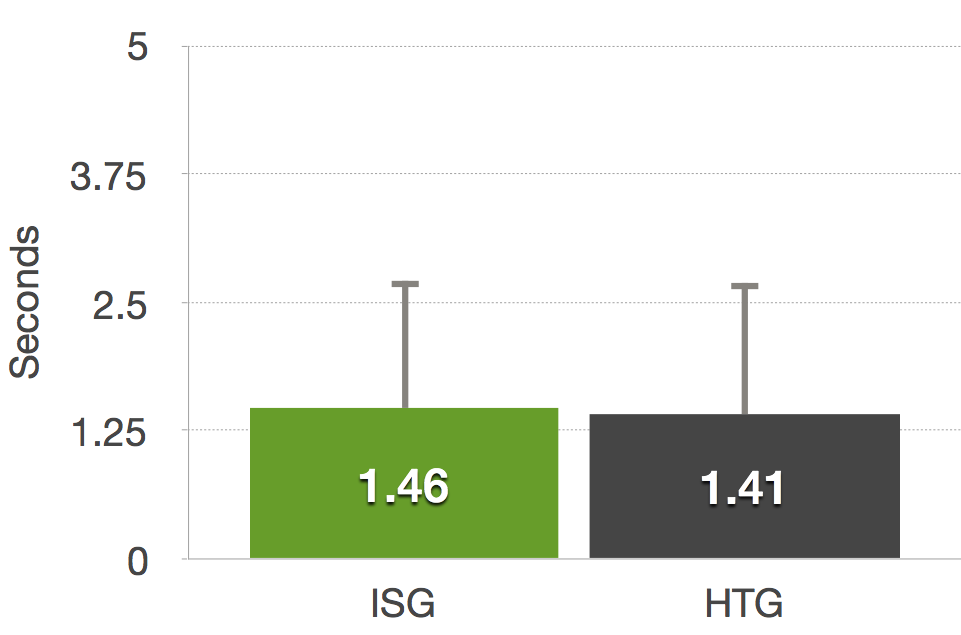
\includegraphics[width=1\linewidth]{Pictures/6_4_DIA_StandRightDiff}
		\subcaption{Improvement on Standing with Right Leg}
		\label{fig:6_4_standRightImprovement}
	\end{minipage}
	\caption{Single Leg Stance Improvement}
	\label{fig:6_4_standImprovement}
\end{figure}


\begin{comment}
\begin{table}[htb]
\centering
\caption{My caption}
\label{my-label}
\resizebox{\textwidth}{!}{%
{\def\arraystretch{1.1}
\begin{tabular}{llrllrlllllll}
\hline
\multicolumn{1}{c}{} & \multicolumn{2}{l}{ISG} &  & \multicolumn{2}{l}{HTG} &  & \multicolumn{6}{l}{Main Effect} \\ \cline{2-3} \cline{5-6} \cline{8-13} 
 & PRE & \multicolumn{1}{l}{POST} &  & PRE & \multicolumn{1}{l}{POST} &  & G x T & $\eta_{p}^{2}$ & T & $\eta_{p}^{2}$ & G & $\eta_{p}^{2}$ \\ \hline
\tab Stand Left (sec) & \multicolumn{1}{r}{4.92 (1.80)} & 6.64 (2.60) & \multicolumn{1}{r}{} & \multicolumn{1}{r}{5.21 (2.25)} & 6.53 (1.65) & \multicolumn{1}{r}{} & p = 0.798 & 0.007 & p = 0.078 & 0.278 & p = 0.928 & 0.001 \\
\tab Stand Right (sec) & \multicolumn{1}{r}{6.44 (2.02)} & 7.90 (2.33) & \multicolumn{1}{r}{} & \multicolumn{1}{r}{6.35 (2.92)} & 7.76 (2.16) & \multicolumn{1}{r}{} & p = 0.950 & 0.000 & \textbf{p = 0.003} & \textbf{0.609} & p = 0.931 & 0.001
\end{tabular}%
}
}
\end{table}
\end{comment}

\subsection{Walked Steps Performance}
The homogeneity of error variances was given for the single leg performance for the left and right leg, as assessed by Levene's test with $p$ > 0.05.
There was also homogeneity of covariances, as assessed by Box's test for the left ($p$ = 0.831) and right leg ($p$ = 0.420).

There was no statistically significant interaction effect between time and group, for the left ($F$(1.0, 10.0) = 0.044, p = 0.838, partial $\eta_{p}^{2}$ = 0.004) as well as for the right leg ($F$(1.0, 10.0) = 1.039, p = 0.332, partial $\eta_{p}^{2}$ = 0.094) (see Figure \ref{fig:6_4_stepsImprovement}).
Since no statistical significant interaction effect has been found, the main effects within the tests of within-subject effects will be reported.

There was a large statistically significant main effect within-subjects for time (PRE to POST) for the left leg, ($F$(1.0, 10.0) = 15.868, p = 0.003, partial $\eta_{p}^{2}$ = 0.613) and also for the right leg ($F$(1.0, 10.0) = 12.519, p = 0.037, partial $\eta_{p}^{2}$ = 0.367).

No significant main effect between-subjects for group (ISG to HTG) was found for the left ($F$(1.0, 10.0) = 0.753, p = 0.406, partial $\eta_{p}^{2}$ = 0.070) and right leg ($F$(1.0, 10.0) = 0.351, p = 0.567, partial $\eta_{p}^{2}$ = 0.034).
\begin{figure}[htb]
	\centering
	\begin{minipage}[t]{0.49\linewidth}
		\centering
		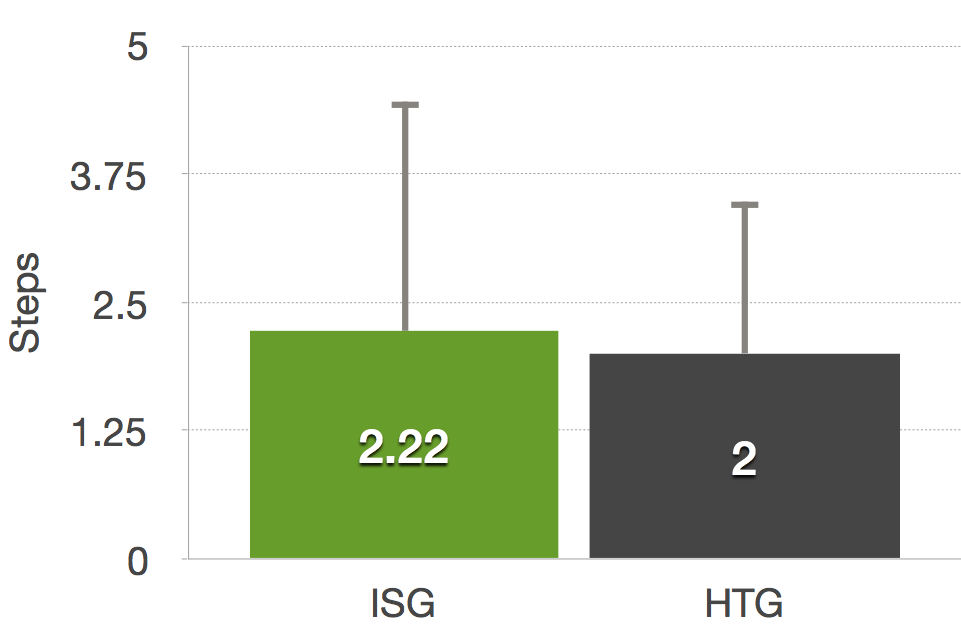
\includegraphics[width=1\linewidth]{Pictures/6_4_DIA_StepsLeftDiff}
		\subcaption{Improvement on Steps with Left Starting Leg}
		\label{fig:6_4_stepsLeftImprovement}
	\end{minipage}
	\hfill
	\begin{minipage}[t]{0.49\linewidth}
		\centering
		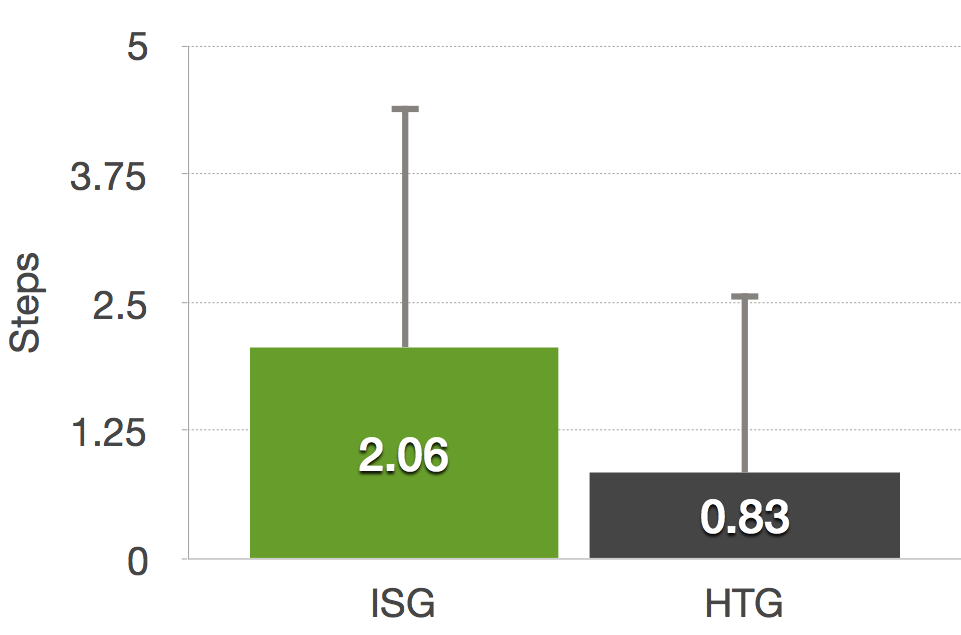
\includegraphics[width=1\linewidth]{Pictures/6_4_DIA_StepsRightDiff}
		\subcaption{Improvement on Steps with Right Starting Leg}
		\label{fig:6_4_stepsRightImprovement}
	\end{minipage}
	\caption{Walked Steps Improvement}
	\label{fig:6_4_stepsImprovement}
\end{figure}

\begin{comment}
\begin{table}[htb]
\centering
\caption{My caption}
\label{my-label}
\resizebox{\textwidth}{!}{%
{\def\arraystretch{1.1}
\begin{tabular}{llrllrlllllll}
\hline
\multicolumn{1}{c}{} & \multicolumn{2}{l}{ISG} &  & \multicolumn{2}{l}{HTG} &  & \multicolumn{6}{l}{Main Effect} \\ \cline{2-3} \cline{5-6} \cline{8-13} 
 & PRE & \multicolumn{1}{l}{POST} &  & PRE & \multicolumn{1}{l}{POST} &  & G x T & $\eta_{p}^{2}$ & T & $\eta_{p}^{2}$ & G & $\eta_{p}^{2}$ \\ \hline
\tab Steps Left & \multicolumn{1}{r}{2.44 (1.26)} & 4.66 (1.53) & \multicolumn{1}{r}{} & \multicolumn{1}{r}{2.06 (1.00)} & 4.06 (1.56) & \multicolumn{1}{r}{} & p = 0.838 & 0.004 & \textbf{p = 0.003} & \textbf{0.613} & p = 0.406 & 0.070 \\
\tab Steps Right & \multicolumn{1}{r}{2.33 (1.05)} & 4.39 (2.00) & \multicolumn{1}{r}{} & \multicolumn{1}{r}{2.61 (1.48)} & 3.44 (0.89) & \multicolumn{1}{r}{} & p = 0.332 & 0.037 & \textbf{p = 0.037} & \textbf{0.367} & p = 0.567 & 0.034
\end{tabular}%
}
}
\end{table}
\end{comment}

\subsection{Walked Distance Performance}
The homogeneity of error variances was given for the single leg performance for the left and right leg, as assessed by Levene's test with $p$ > 0.05.
There was also homogeneity of covariances, as assessed by Box's test for the left ($p$ = 0.712) and right leg ($p$ = 0.193).

There was no statistically significant interaction effect between time and group, for the left ($F$(1.0, 10.0) = 0.006, p = 0.942, partial $\eta_{p}^{2}$ = 0.001) as well as for the right leg ($F$(1.0, 10.0) = 1.235, p = 0.292, partial $\eta_{p}^{2}$ = 0.110) (see Figure \ref{fig:6_4_distanceImprovement}).
Since no statistical significant interaction effect has been found, the main effects within the tests of within-subject effects will be reported.

In terms of within-subject time (PRE to POST) a large statistically significant main effect has been found for the left leg ($F$(1.0, 10.0) = 18.563, p = 0.002, partial $\eta_{p}^{2}$ = 0.650) and also for the right leg ($F$(1.0, 10.0) = 7.082, p = 0.024, partial $\eta_{p}^{2}$ = 0.415).

No significant main effect between-subjects for group (ISG to HTG) was found for the left ($F$(1.0, 10.0) = 0.399, p = 0.542, partial $\eta_{p}^{2}$ = 0.038) and right leg ($F$(1.0, 10.0) = 0.145, p = 0.711, partial $\eta_{p}^{2}$ = 0.014).
\begin{figure}[htb]
	\centering
	\begin{minipage}[t]{0.49\linewidth}
		\centering
		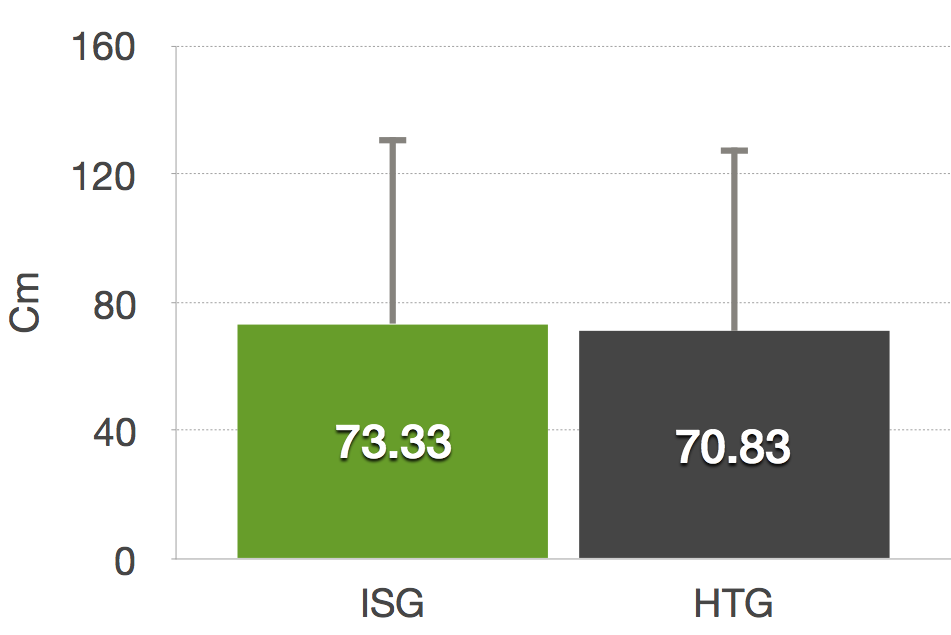
\includegraphics[width=1\linewidth]{Pictures/6_4_DIA_DistanceLeftDiff}
		\subcaption{Improvement on Distance with Left Starting Leg}
		\label{fig:6_4_distanceLeftImprovement}
	\end{minipage}
	\hfill
	\begin{minipage}[t]{0.49\linewidth}
		\centering
		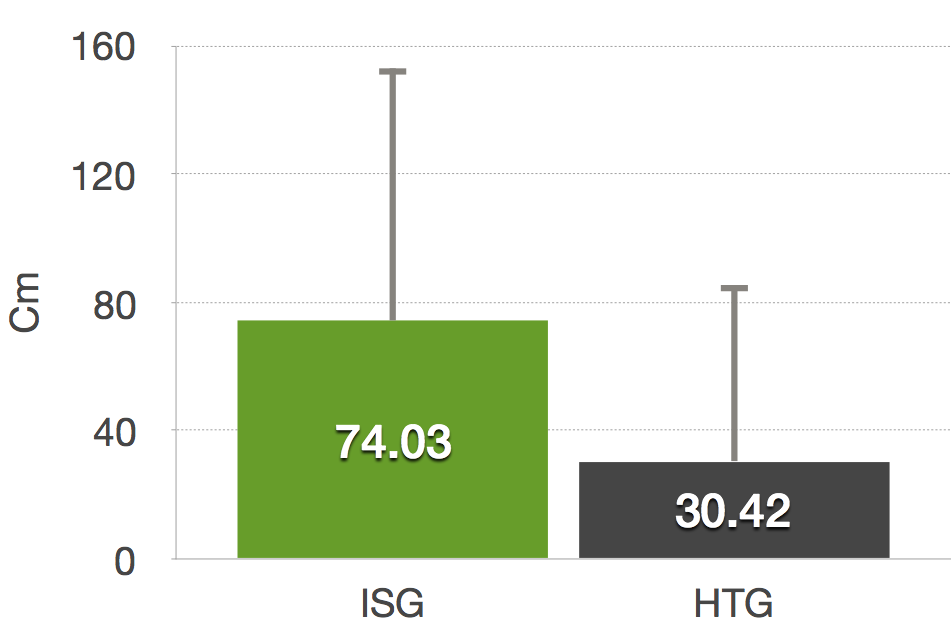
\includegraphics[width=1\linewidth]{Pictures/6_4_DIA_DistanceRightDiff}
		\subcaption{Improvement on Distance with Right Starting Leg}
		\label{fig:6_4_distanceRightImprovement}
	\end{minipage}
	\caption{Walked Distance Improvement}
	\label{fig:6_4_distanceImprovement}
\end{figure}

\begin{comment}
\begin{table}[htb]
\centering
\caption{My caption}
\label{my-label}
\resizebox{\textwidth}{!}{%
{\def\arraystretch{1.1}
\begin{tabular}{llrllrlllllll}
\hline
\multicolumn{1}{c}{} & \multicolumn{2}{l}{ISG} &  & \multicolumn{2}{l}{HTG} &  & \multicolumn{6}{l}{Main Effect} \\ \cline{2-3} \cline{5-6} \cline{8-13} 
 & PRE & \multicolumn{1}{l}{POST} &  & PRE & \multicolumn{1}{l}{POST} &  & G x T & $\eta_{p}^{2}$ & T & $\eta_{p}^{2}$ & G & $\eta_{p}^{2}$ \\ \hline
\tab Distance Left (cm) & \multicolumn{1}{r}{112.92 (35.90)} & 186.25 (43.25) & \multicolumn{1}{r}{} & \multicolumn{1}{r}{101.67 (28.46)} & 172.50 (63.94) & \multicolumn{1}{r}{} & p = 0.942 & 0.001 & \textbf{p = 0.002} & \textbf{0.650} & p = 0.542 & 0.038 \\
\tab Distance Right (cm) & \multicolumn{1}{r}{105.14 (25.30)} & 179.17 (66.65) & \multicolumn{1}{r}{} & \multicolumn{1}{r}{119.17 (56.86)} & 149.58 (36.13) & \multicolumn{1}{r}{} & p = 0.292 & 0.110 & \textbf{p = 0.024} & \textbf{0.415} & p = 0.711 & 0.014 \\ \hline
\end{tabular}%
}
}
\end{table}
\end{comment}

% Please add the following required packages to your document preamble:
% \usepackage{graphicx}
\begin{table}[htb]
\centering
\caption{Means and standard deviation results for single leg stance, walked steps, and walked distance in the interactive system group (ISG) and human trainer group (HTG)}
%\caption{PRE and POST mean and SD values for each condition (ISG and HTG) and measurement variable}
\label{tab:6_4_results}
\resizebox{\textwidth}{!}{%
{\def\arraystretch{1.1}
\begin{tabular}{lrrrrr}
\hline
\multicolumn{1}{c}{} & \multicolumn{2}{l}{ISG} & \multicolumn{1}{l}{} & \multicolumn{2}{l}{HTG} \\ \cline{2-3} \cline{5-6} 
 & \multicolumn{1}{l}{PRE} & \multicolumn{1}{l}{POST} & \multicolumn{1}{l}{} & \multicolumn{1}{l}{PRE} & \multicolumn{1}{l}{POST} \\ \hline
Stand Left (sec) & 4.92 (1.80) & 6.64 (2.60) &  & 5.21 (2.25) & 6.53 (1.65) \\
Stand Right (sec) & 6.44 (2.02) & 7.90 (2.33) &  & 6.35 (2.92) & 7.76 (2.16) \\
Steps Left & 2.44 (1.26) & 4.66 (1.53) &  & 2.06 (1.00) & 4.06 (1.56) \\
Steps Right & 2.33 (1.05) & 4.39 (2.00) &  & 2.61 (1.48) & 3.44 (0.89) \\
Distance Left (cm) & 112.92 (35.90) & 186.25 (43.25) &  & 101.67 (28.46) & 172.50 (63.94) \\
Distance Right (cm) & 105.14 (25.30) & 179.17 (66.65) &  & 119.17 (56.86) & 149.58 (36.13) \\ \hline
\end{tabular}%
}
}
\end{table}

% Please add the following required packages to your document preamble:
% \usepackage{graphicx}
\begin{table}[htb]
\centering
\caption{Interaction, time, and group effects on single leg stance, walking steps, and walked distance}
%\caption{Significance value and effect sizes ($\eta_{p}^{2}$) for interaction effects, time, and group}
\label{tab:6_4_mainEffects}
\resizebox{\textwidth}{!}{%
{\def\arraystretch{1.1}
\begin{tabular}{lllllll}
\hline
\multicolumn{1}{c}{} & \multicolumn{6}{l}{Main Effect} \\ \cline{2-7} 
 & Group x Time & $\eta_{p}^{2}$ & Time & $\eta_{p}^{2}$ & Group & $\eta_{p}^{2}$ \\ \hline
Stand Left (sec) & p = 0.798 & 0.007 & p = 0.078 & 0.278 & p = 0.928 & 0.001 \\
Stand Right (sec) & p = 0.950 & 0.000 & \textbf{p = 0.003} & \textbf{0.609} & p = 0.931 & 0.001 \\
Steps Left & p = 0.838 & 0.004 & \textbf{p = 0.003} & \textbf{0.613} & p = 0.406 & 0.070 \\
Steps Right & p = 0.332 & 0.037 & \textbf{p = 0.037} & \textbf{0.367} & p = 0.567 & 0.034 \\
Distance Left (cm) & p = 0.942 & 0.001 & \textbf{p = 0.002} & \textbf{0.650} & p = 0.542 & 0.038 \\
Distance Right (cm) & p = 0.292 & 0.110 & \textbf{p = 0.024} & \textbf{0.415} & p = 0.711 & 0.014 \\ \hline
\end{tabular}%
}
}
\end{table}

\subsection{Observations of the User Study}\label{results_interview}
In the pre measurement all participants had no real control of their body during standing and walking over the slackline.
Furthermore, they tried to walk fast over the slackline.
The post measurement, after the training, showed that each participant improved to stand and walk slowly and with a certain sense of body control on the line.

All participant had fun during the training and enjoyed to play with the system.
They were positively surprised by the tracking ability of the Kinect.

The checklist seen in Figure~\ref{fig:6_5_sittingProblems} at the left side above the repetitions and the coloured timer on the mid right side, were mentioned as very useful feedback indicator.

Participants were also motivated to accomplish the current exercises for unlocking the next excises.

Beside these, there were also a number of problems that occured.
In the case of general tracking performance with the Kinect there existed problems with the clothing color of a participant.
She showed up with black clothes, with which the Kinect had problems to detect her.
This is because black clothing absorb the infrared light of the Kinect that makes the tracking ability more difficult \cite{KinectBlackClothing}.

Concerning the exercises during the training problems occurred with the gesture detection while sitting on the slackline for five out of six participants.
Like seen in the user view of Figure~\ref{fig:6_5_sittingProblems}, the leg of the participant was wrongly tracked.
With other participants their leg was often mistaken with the slackline by the Kinect.
All participants of both groups noted also that the sitting exercises are very uncomfortable.
\begin{figure}[htb]
	\centering
	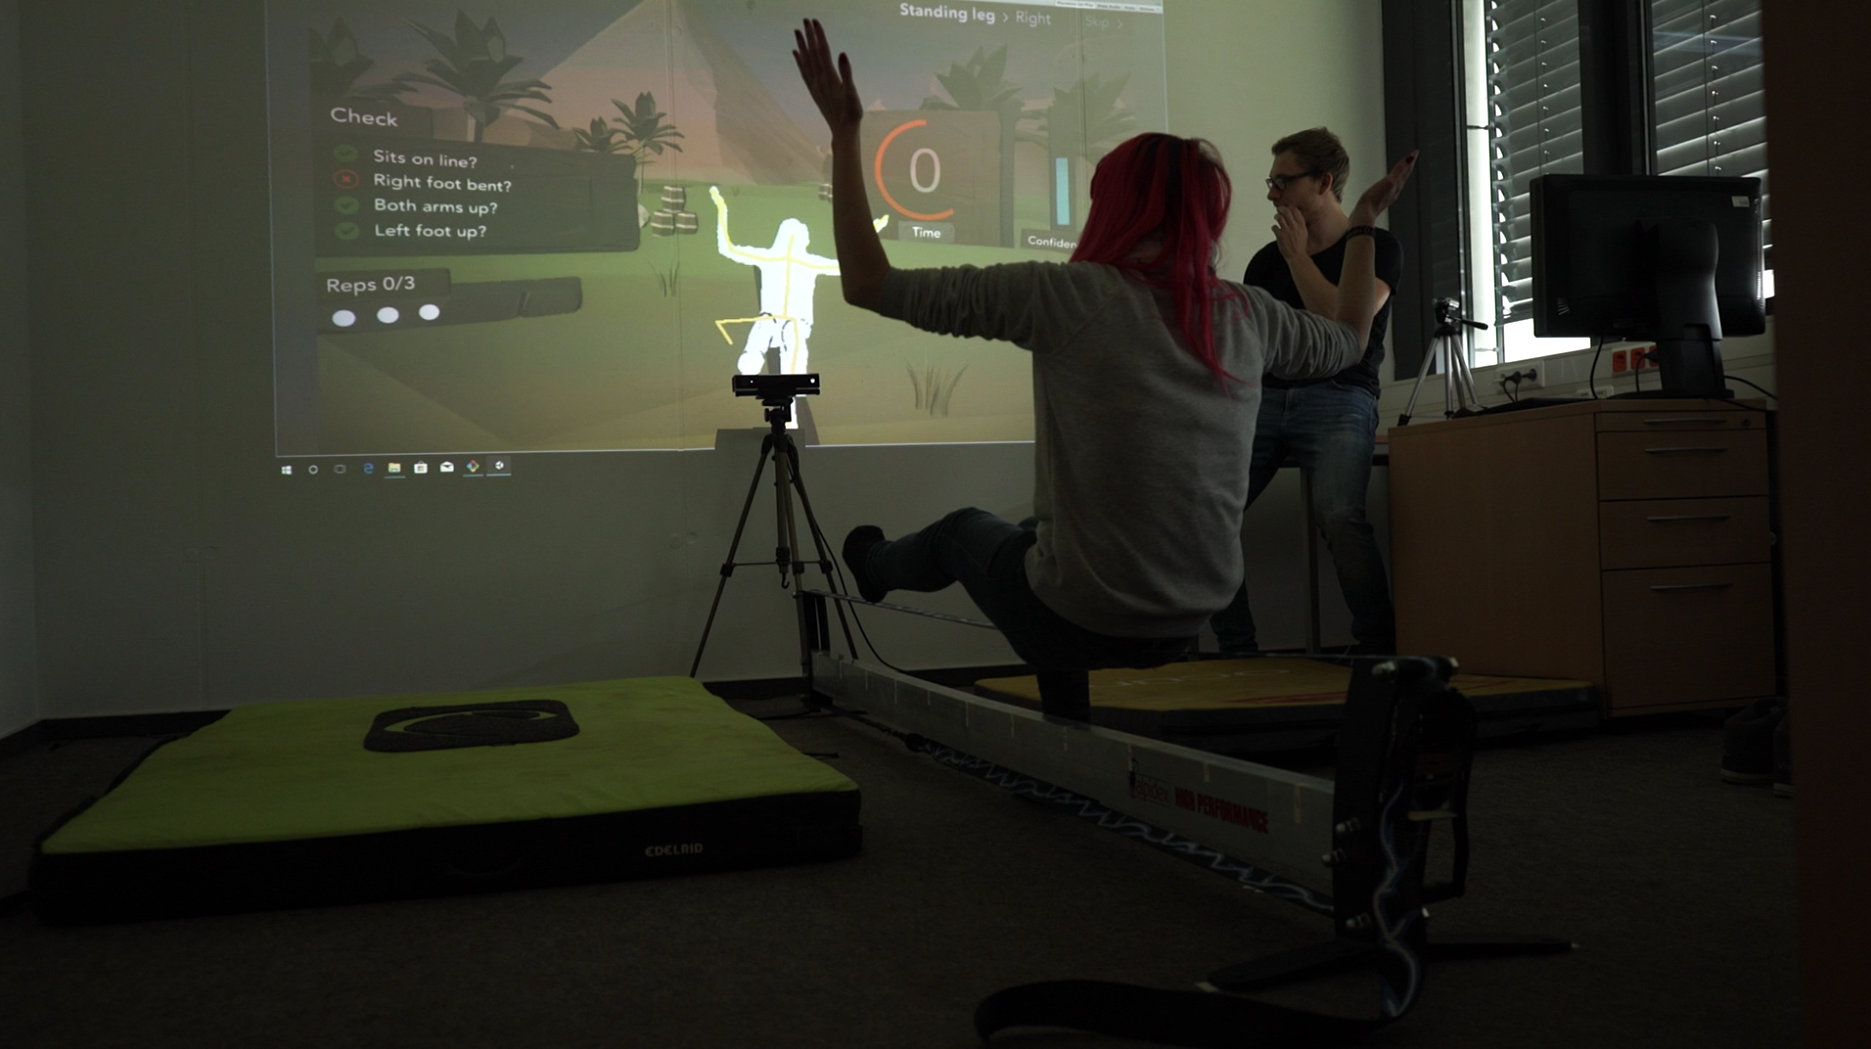
\includegraphics[width=0.97\linewidth]{Pictures/6_5_sitting}
	\caption{The leg of the participant is wrongly tracked by the Kinect, which caused problems for the participant to finish the exercise}
	\label{fig:6_5_sittingProblems}
\end{figure}

The very last exercise resulted also in tracking problems with four out of six participants.
Here, the participants had to walk two steps forward on the slackline and hold the end pose for a half second.

A general problem was going up on the slackline.
When the participant put her outer leg too close to the line while going up, the Kinect did not tracked it appropriately.
The exercise execution was therefore sometimes not successfully counted.

Three participants in the ISG had small problems with the interaction of the system.
Especially with scrolling the exercise list at the beginning, because they didn't know how to interact with it.

\subsection{Rating of Exercise Difficulty}
Participants were asked to rate each exercises after finishing a set of exercises with both legs.
They could choose a difficulty on a scale from 1 (very easy) to 5 (very difficult).
The ratings of all participants were averaged.
Figure \ref{fig:6_4_exerciseDifficulty} shows the ratings of each exercise (blue line) as well as a trendline, which is a linear interpolation of the values (green line), and the standard deviation of each rating (grey bars).

\begin{figure}[htb]
	\centering
	\begin{minipage}[t]{1\linewidth}
		\centering
		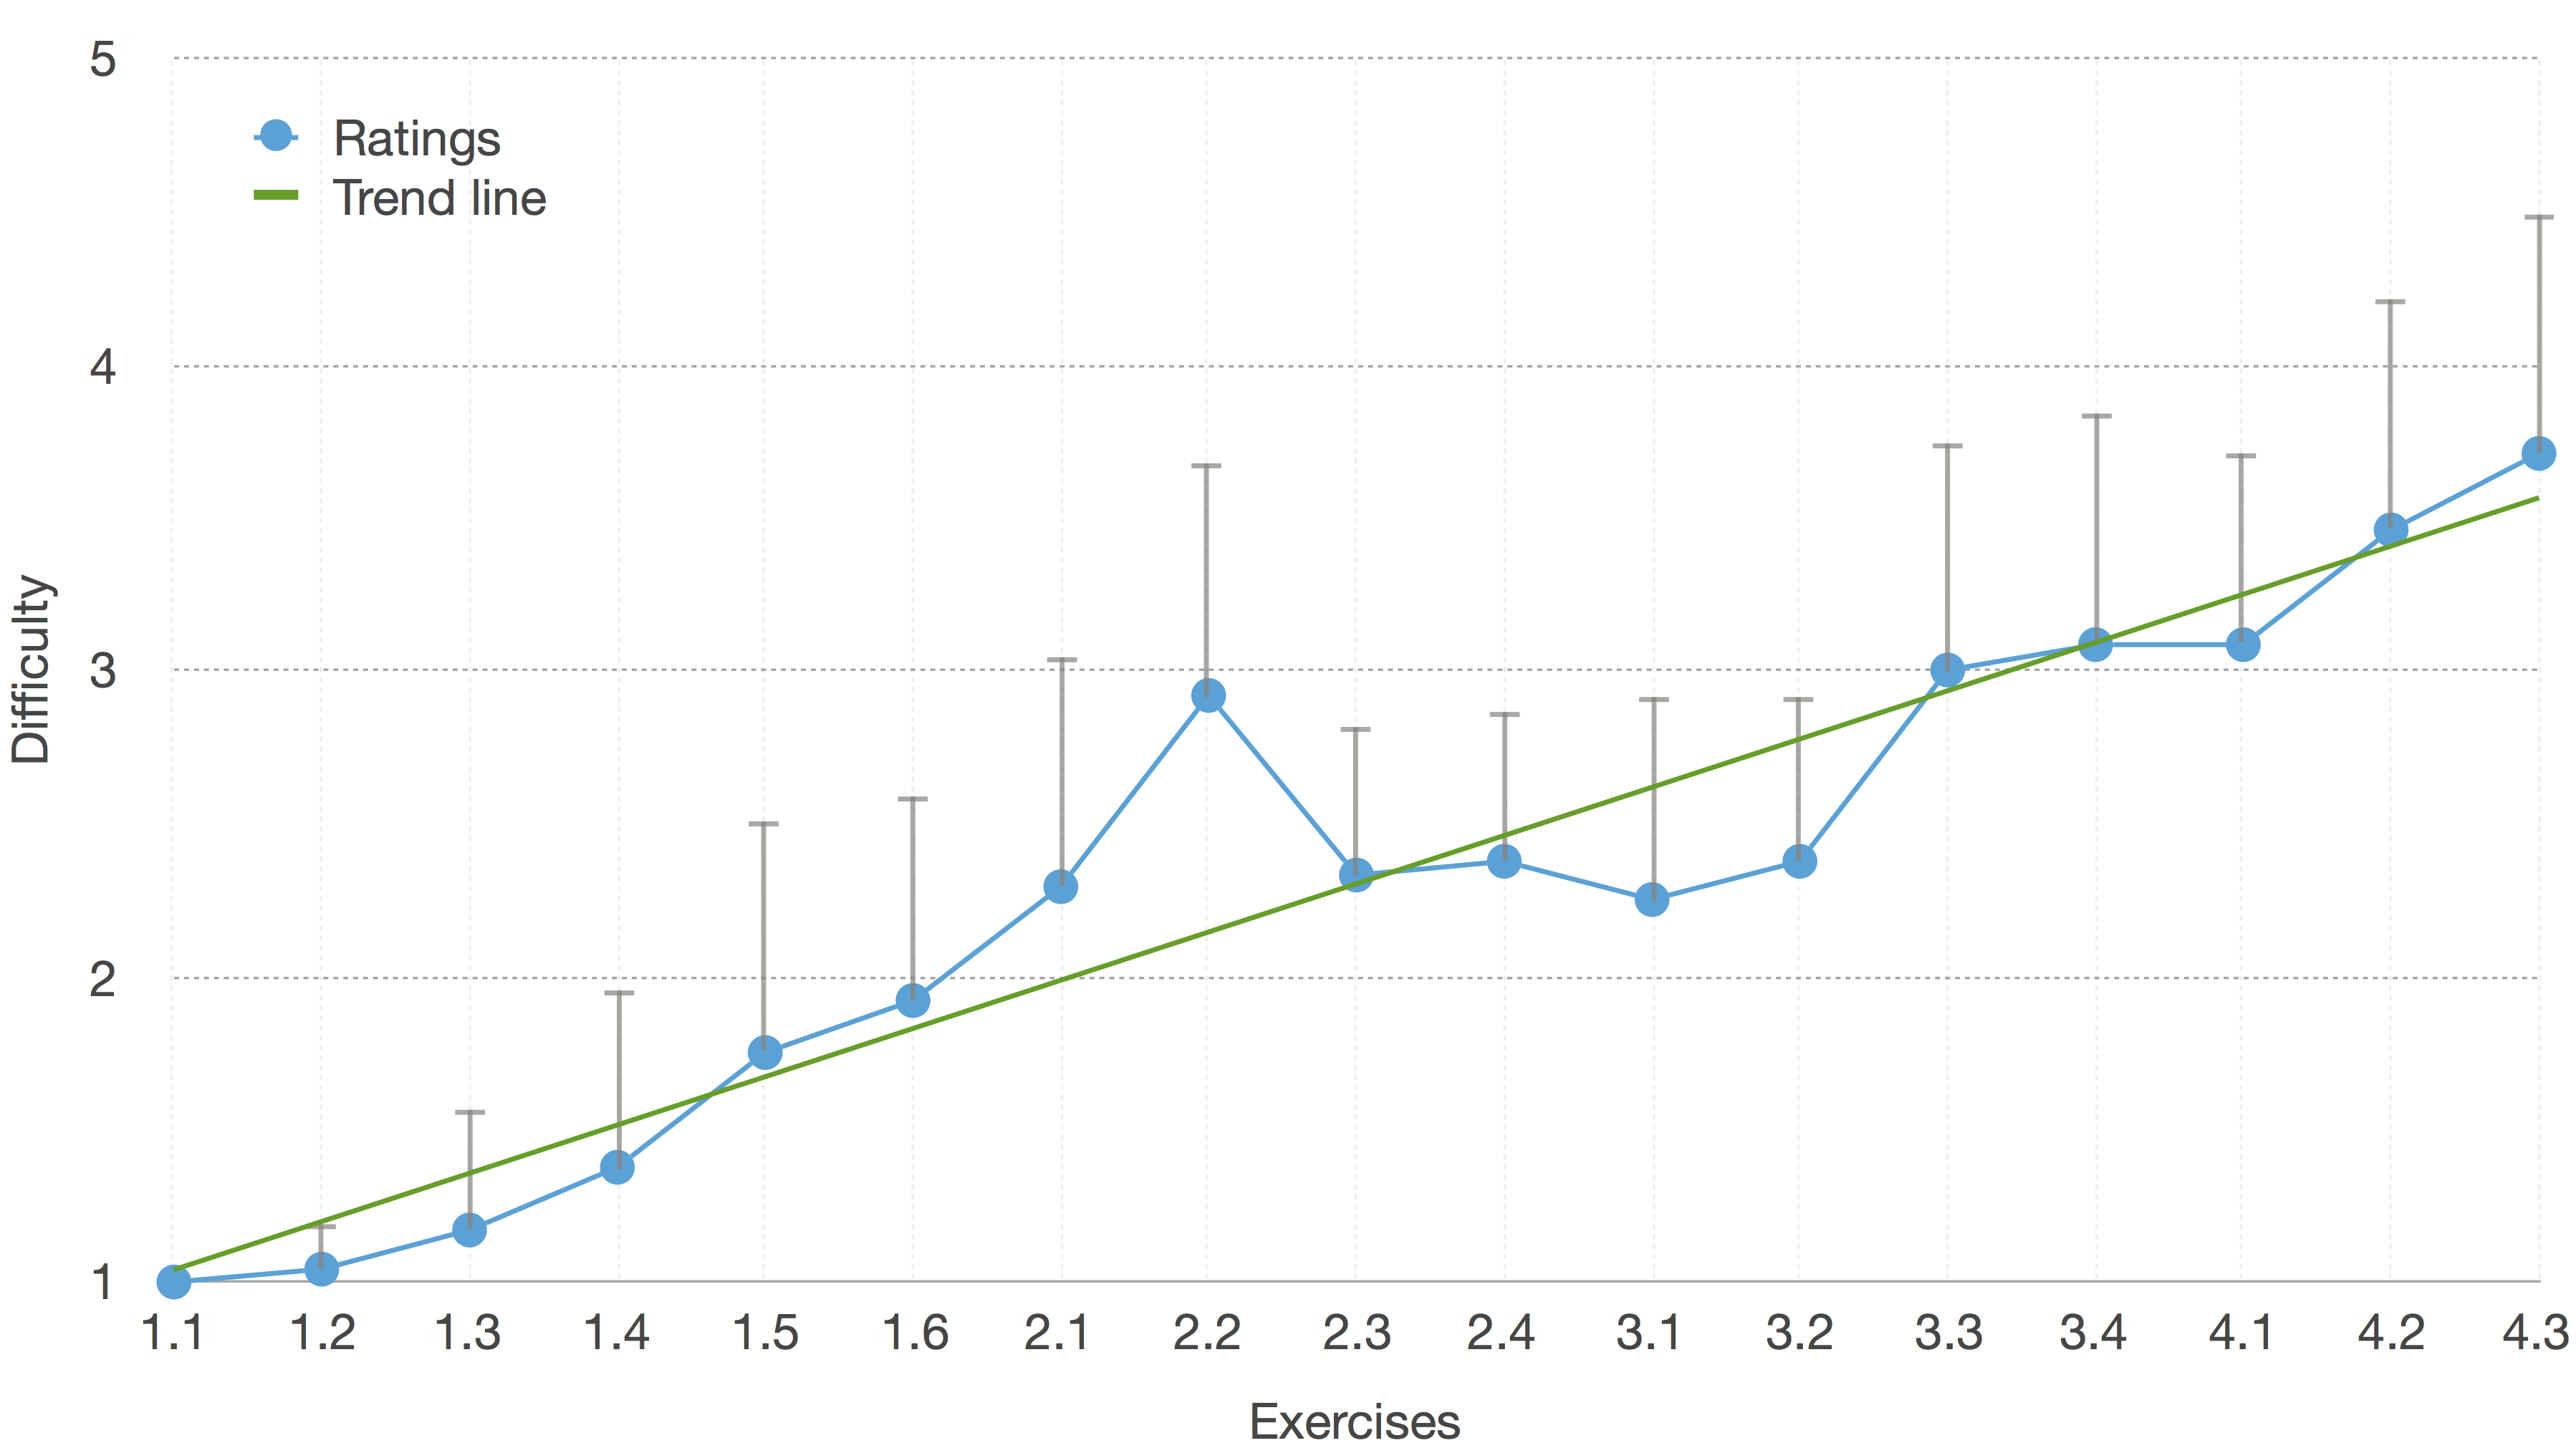
\includegraphics[width=1\linewidth]{Pictures/6_4_DIA_ExerciseDifficulty2}
		\caption{Averaged exercise difficulty rating of the participants. Blue points: Rating, Green line: Trend line, Grey bars: Standard deviation}
		\label{fig:6_4_exerciseDifficulty}
	\end{minipage}
\end{figure}

The exercises of the first level follow a smooth increase in difficulty.
For the second level there is a massive increase in difficulty for the first two exercises.
The ratings for the exercises 2.3, 2.4, 3.1, and 3.2 show comparable difficulty results, since they were the same but exercise 3.1 and 3.2 were different in the time the user has to hold the exercise.
Furthermore, the ratings follow a linear ongoing trend.

\subsection{Semi-Structured Interview}
The general experience with the training method showed similar outcomes for both groups. 
They mentioned a positive learning progress during the training and had a sense of achievement through challenging but practicable exercises.
%Representative participant 10 said: \textit{"The Exercises were well-framed. I felt a learning progress. At the beginning i was not aware of the whole body balance but after the training it could feel how the body balance changed and how I could keep my body in the center of gravity."}

All participants in the ISG liked the environment design, clear description, and especially the looping videos of the exercises as well as the appropriate feedback during the execution.
Participant 6 said further \textit{"I liked the user view because you can see how you act by yourself. It is also positive that I can use the system without any further help."}

Participant 3 (ISG) mentioned \textit{"[...]~There is no need to watch YouTube tutorials with such a system. It displays all relevant information and provides appropriate feedback"}.
Participant 4 and 6 (ISG) said a personal trainer could be more helpful due to the fact for giving more specific advises, which the Kinect could not detect.
%answered \textit{"Yes because I have learned something and I do not have to watch YouTube tutorials because it tells me whether I am wrong or not. The user view is also helpful during the exercise execution"}. Participant 4 (ISG) mentioned \textit{"For beginners very well because you can feel and see your own progress through unlocking the exercises. Although a personal trainer could mention things that the Kinect won't detect"}.

The most annoying experience for the ISG was the partially bad gesture recognition of the Kinect and the interaction with it.
Participant 10 of the HTG mentioned missing exercises for how to get up on the slackline and participant 12 noted especially the uncomfortableness of the sitting on the slackline exercises.

Lastly, a various amount of application scenarios for the interactive training system were mentioned.
Among others the most stated were physiotherapy, rehabilitation, in general as training for sport activities, gym, and home trainer.


\begin{comment}
%{\def\arraystretch{1.1}

% Please add the following required packages to your document preamble:
% \usepackage{graphicx}
\begin{table}[htb]
\centering
\caption{}
\label{my-label}
\resizebox{\textwidth}{!}{%
{\def\arraystretch{1.1}
\begin{tabular}{lrrrrrrllllll}
\hline
\multicolumn{1}{c}{} & \multicolumn{2}{l}{ISG} & \multicolumn{1}{l}{} & \multicolumn{2}{l}{HTG} & \multicolumn{1}{l}{} & \multicolumn{6}{l}{Main Effect} \\ \cline{2-3} \cline{5-6} \cline{8-13} 
 & \multicolumn{1}{l}{PRE} & \multicolumn{1}{l}{POST} & \multicolumn{1}{l}{} & \multicolumn{1}{l}{PRE} & \multicolumn{1}{l}{POST} & \multicolumn{1}{l}{} & G x T & $\eta_{p}^{2}$ & T & $\eta_{p}^{2}$ & G & $\eta_{p}^{2}$ \\ \hline
\tab Stand Left (sec) & 4.92 (1.80) & 6.64 (2.60) &  & 5.21 (2.25) & 6.53 (1.65) &  & p = 0.798 & 0.007 & p = 0.078 & 0.278 & p = 0.928 & 0.001 \\
\tab Stand Right (sec) & 6.44 (2.02) & 7.90 (2.33) &  & 6.35 (2.92) & 7.76 (2.16) &  & p = 0.950 & 0.000 & \textbf{p = 0.003} & \textbf{0.609} & p = 0.931 & 0.001 \\
\tab Steps Left & 2.44 (1.26) & 4.66 (1.53) &  & 2.06 (1.00) & 4.06 (1.56) &  & p = 0.838 & 0.004 & \textbf{p = 0.003} & \textbf{0.613} & p = 0.406 & 0.070 \\
\tab Steps Right & 2.33 (1.05) & 4.39 (2.00) &  & 2.61 (1.48) & 3.44 (0.89) &  & p = 0.332 & 0.037 & \textbf{p = 0.037} & \textbf{0.367} & p = 0.567 & 0.034 \\
\tab Distance Left (cm) & 112.92 (35.90) & 186.25 (43.25) &  & 101.67 (28.46) & 172.50 (63.94) &  & p = 0.942 & 0.001 & \textbf{p = 0.002} & \textbf{0.650} & p = 0.542 & 0.038 \\
\tab Distance Right (cm) & 105.14 (25.30) & 179.17 (66.65) &  & 119.17 (56.86) & 149.58 (36.13) &  & p = 0.292 & 0.110 & \textbf{p = 0.024} & \textbf{0.415} & p = 0.711 & 0.014 \\ \hline
\end{tabular}%
}
}
\end{table}
\end{comment}

\begin{comment}
\subsection{Two-Tailed Paired-Samples T-Test}
At first will be checked if there are any outliers in the dataset.
Then the results for the normal distribution of each performance condition will be stated since it is a requirement for the two-tailed paired-samples t-test.
After that the results of the significance will be stated.
In the following the outcomes for the single leg stance as well as the steps and distance walked over the slackline will be reported.

\subsubsection{Single Leg Stance Performance}
There were no outliers in the data.
The differences between the pre- and post-scores for the single leg stance were normally distributed, as assessed by the Shapiro-Wilk test for the left leg ($p$ = 0.987) as well as for the right leg ($p$ = 0.203).
There was no difference in single leg stance scores for the left leg before and after the training (t(11) = -2.05, $p$ = 0.065).
The wilcoxon signed ranks test also showed no significant difference (exact significance: $z$ = -1.80, $p$ = 0.077).
Single leg stance score for the right leg was significantly higher after the training (t(11) = -4.14, $p$ = 0.002).
A significant difference was also shown by the wilcoxon signed ranks test (exact significance: $z$ = -2.75, $p$ = 0.003).

\todo{table with means and SD}

\subsubsection{Walked Steps Over the Line Performance}
There were no outliers in the data.
The differences between the pre- and post-scores for the counted steps when walking over the line were normally distributed, as assessed by the Shapiro-Wilk test for the left leg ($p$ = 0.613) as well as for the right leg ($p$ = 0.099).
Steps over the line scores were significantly higher after the training for the left leg, $t$(11) = -4.17, $p$ = 0.002 and for the right leg, $t$(11) = -2.41, $p$ = 0.035.
The wilcoxon signed ranks test also showed significant difference for the left leg (exact significance: $z$ = -2.95, $p$ = 0.001) and for the right leg (exact significance: $z$ = -2.09, $p$ = 0.034).

\todo{table with means and SD}

\subsubsection{Walked Distance Over the Line Performance}
There were no outliers in the data.
The differences between the pre- and post-scores for the distance walked over the line were normally distributed, as assessed by the Shapiro-Wilk test for the left leg ($p$ = 0.358) as well as for the right leg ($p$ = 0.104).
Distance walked over the line scores were significantly higher after the training for the left leg $t$(11) = -4.52, $p$ = 0.001 and for the right leg, $t$(11) = -2.63, $p$ = 0.023.
The wilcoxon signed ranks test also showed significant difference for the left leg (exact significance: $z$ = -2.98, $p$ = 0.001) and for the right leg (exact significance: $z$ = -2.35, $p$ = 0.016).

\todo{table with means and SD}

\subsection{Independent-Samples T-Test}


\subsubsection{Single Leg Stance Performance}

\subsubsection{Walked Steps Over the Line Performance}

\subsubsection{Walked Distance Over the Line Performance}
\end{comment}
